\documentclass[bwprint, withoutpreface]{cumcmthesis}

\usepackage{extarrows}
\usepackage{authblk}
\usepackage{tikz}

\title{实变第一章总结}

\begin{document}
\maketitle
\noindent Author: Tony Xiang

\noindent Full Document can be acquired here: 

\noindent https://github.com/T0nyX1ang/RealAnaly-Documents/blob/master/Chapter\%201/Chapter1.pdf

\noindent Full Source code can be downloaded here:

\noindent https://github.com/T0nyX1ang/RealAnaly-Documents/blob/master/Chapter\%201/Chapter1.tex

\section{集合与集合的运算}
\indent 集合的表示:列举法,描述法.

子集,真子集.

\textbf{幂集:} $\mathcal{P}(X) = \{A:A \subset X\}$, 若$|X|=n$,则$|\mathcal{P}(X)|=2^n$.

集合的有限交,并,差,余.

相对差集:$A \Delta B = (A - B) \cup (B - A)$,若$A \Delta B = \emptyset$,$A = B$.

集族,集列:若对$\forall \alpha \in I$都对应一个集$A_{\alpha}$,则称$\{A_n\}_{\alpha \in I}$为集族.若$I = \mathbb{N}$,则称$\{A_n\}_{\alpha \in \mathbb{N}}$为集列.

集合的可列交:
\begin{equation*}
	\bigcup_{\alpha \in I}{A_\alpha} = \{\exists \alpha \in I, s.t. \quad x \in A_{\alpha}\}
\end{equation*}.

集合的可列并:
\begin{equation*}
	\bigcap_{\alpha \in I}{A_\alpha} = \{\forall \alpha \in I, x \in A_{\alpha}\}
\end{equation*}.

可列交与可列并的性质:交换律,结合律,分配律.

\textbf{De Morgan 公式:}
\begin{align*}
	{(\bigcup_{\alpha \in I}{A_{\alpha}})}^C = \bigcap_{\alpha \in I}{{A_{\alpha}}^C} \\ 
	{(\bigcap_{\alpha \in I}{A_{\alpha}})}^C = \bigcup_{\alpha \in I}{{A_{\alpha}}^C}
\end{align*}

\textbf{集合的表示:}根据所给条件由内向外进行表示.一般等价转化为:$\forall: \bigcap$,$\exists: \bigcup$.通过对\textbf{指标依赖的分析},依次将极限定义转化为集合符号的定义。

直积:有序$n$元组全体构成的集:$\{ (x_1, x_2, \cdots, x_n): x_1 \in A_1, x_2 \in A_2, \cdots, x_n \in A_n \}$

集列的极限:

上极限:
\begin{equation*}
	\varlimsup_{n \to \infty} = \{x: x\mbox{属于}A_n\mbox{中的无限多个}\}
\end{equation*}.

下极限:
\begin{equation*}
	\varliminf_{n \to \infty} = \{x: x\mbox{至多不属于}A_n\mbox{中的有限多个}\}
\end{equation*}.

\begin{equation*}
	\varlimsup_{n \to \infty} \subset \varliminf_{n \to \infty}
\end{equation*}

若
\begin{equation*}
	\varlimsup_{n \to \infty} = \varliminf_{n \to \infty}
\end{equation*}

则称$\{A_n\}$存在极限,记
\begin{equation*}
	A \xlongequal{def} \varlimsup_{n \to \infty} = \varliminf_{n \to \infty}
\end{equation*}

\textbf{集列极限的表示:上极限先变大再变小,下极限先变小再变大.}
\begin{align*}
	\varlimsup_{n \to \infty} = \bigcap_{n = 1}^{\infty}{\bigcup_{k = n}^{\infty}{A_k}} \\
	\varliminf_{n \to \infty} = \bigcup_{n = 1}^{\infty}{\bigcap_{k = n}^{\infty}{A_k}}
\end{align*}

\textbf{单调集列必存在极限,且:}
\begin{align*}
	\lim{A_n} = \bigcup_{n = 1}^{\infty}{A_n} \quad A_n\mbox{单调递减} \\
	\lim{A_n} = \bigcap_{n = 1}^{\infty}{A_n} \quad A_n\mbox{单调递增}
\end{align*}

\section{映射,可列集,基数}
\indent 映射,值域,定义域,像,原像,函数,单射,满射,双射,逆映射,反函数,复合映射,延拓,限制.

\textbf{特征函数(示性函数):}

$A \subset X$,
\begin{equation*}
	\chi_A(x) = 
	\begin{cases}
		1, \quad x \in A \\
		0, \quad x \not \in A		
	\end{cases}	
\end{equation*}

特征函数的性质.

\textbf{特征函数能够表示分段函数,可以看作对函数的一种“粘连”:}
\begin{equation*}
	f(x) = \sum_{i = 1}^{n}{f_i(x)\chi_{A_i}(x)}
\end{equation*}

其中$\{A_n\}$为不相交的子集,并且$X$为它们的并集.$f_i(x)$为定义在$\{A_i\}$上的函数。

\textbf{集合的对等关系:}$A$,$B$是两个非空集合,若$\exists \varphi:A \to B, \varphi\mbox{为双射}$,则$A$,$B$对等,记为$A \sim B$.且$\emptyset \sim \emptyset$.

集合的对等关系满足自反性,对称性与传递性.

\textbf{可列集:}与自然数集$\mathbb{N}$对等的集合称为可列集.

\textbf{可列集的等价定义:集$A$是可列集的充要条件是$A$的元素可以编号为一个无穷序列.}即:$A=\{a_1, a_2, \cdots, a_n\}$.编号排序\textbf{不重不漏}.

注意:可列集可以与它的一个真子集对等,而有限集不能。

\textbf{可列集的性质及应用:}

\begin{itemize}[itemindent=2em]
	\item $A$是可列集,$B$是有限集,则$A \cup B$为可列集.这个性质的证明可以通过编号法解决.这可以导出证明一个集合是可列集的一个方法:先构造不交并,然后分而治之.即:$A \cup B = A \cup (B - A), A \cap (B - A) = \emptyset$.作业第2题给出了一般情况下的构造方法.
	\item 可列集的任何无限子集仍是可列集.这个性质的证明可以通过取子列然后编号解决.
	\item 任何无限集包含一个可列的子集.这个性质的证明通过顺序取子列,类似数学归纳法的方式证明.
	\item 可数集的有限并与可列并为可数集.这个性质包含:可列集的有限并与可列并是可列集;有限集的可列并是\textbf{有限集或可列集}.这个性质的证明是通过对元素的合理排列完成的,这是一个比较重要的证明方法.即\textbf{编号法的合理性在于,任取一个元素,能够确定该元素的编号.}比较常见的方法有横排法,竖排法,正方形法与对角线法.
	\item 可列集的直积为可列集.这个性质可以通过集合的分解证明($A_1=\{a_1, a_2, \cdots, a_n\}$,$A_2=\{b_1, b_2, \cdots, b_n\}$,$E_k=A_1 \times \{b_k\}$,$A_1 \times A_2 = \bigcap_{k=1}^{\infty}{E_k}$).这是一个比较重要的证明方法,这个方法的理论基础在于上一个性质:\textbf{可数集的有限并与可列并为可数集.}当然,对于二维的情形,也可以直接采用正方形法或三角形法证明.这个性质的一个推论是,以$n$个元素作直积构成的集合中的元为下标的元的全体构成的集合为可列集.
	\item $\mathbb{Q}, \mathbb{Q}^n, P_n\mbox{(整系数多项式构成的全体)},\mathbb{A}\mbox{(代数数集)}$为可列集.超越数的存在性.
	\item 直线上一族互不相交的开区间所成的集是可数集.这个性质通过构造映射的方法证明.这是一个比较重要的证明方法.通常而言,利用有理数的稠密性与有理数集的可列,将集合与$\mathbb{Q}$对等.一般而言,构造一个映射需要一定的技巧.这个性质的一个推论是:单调函数的间断点的全体是可数集.
\end{itemize}

基数:$A \sim B$,则称$A, B$具有相同的基数(势).集合$A$的基数记为$\overline{\overline{A}}$.

规定集$\{1, 2, \cdots, n\}$的基数为$n$,$\overline{\overline{\emptyset}}=0$.自然数集$\mathbb{N}$的基数用$\aleph_0$表示.实数集$\mathbb{R}$的基数用$c$表示,称之为连续基数.

基数大小的比较.$\aleph_0 < c$.

\textbf{若$A$是无限集,$B$是可数集,则$\overline{\overline{A \cup B}} = \overline{\overline{A}}$}.证明方法为构造一个映射:从$A$中选一个可列的集合$A_1$,将$A_1,B$通过奇偶关系重组到一起.

$\overline{\overline{\mathbb{R}-\mathbb{Q}}} = c$,直线上任何区间的基数都是$c$(转化为$\overline{\overline{(0, 1)}} = c$).

$p$进制小数,可转化为级数的求和.

区间$(0, 1]$中的任一实数可以唯一表示成一个$p$进制无限小数.可以通过区间的分割证明.

二元数列的全体构成的集合的基数为$c$,进一步有:可列集$X$的幂集$\mathcal{P}(X)$的基数为$c$.即$2^{\aleph_0} = c$.

本节之后的内容不作要求.

\section{集类}
\indent 集类: $X$是一个固定的非空集,$X$的满足某个条件的子集的全体所成的集称为$X$上的集类.一般用花体字母$\mathcal{A},\mathcal{B},\mathcal{C}$表示.

集类对运算的封闭性.(可以联系抽代对封闭性的定义)

代数:$\mathcal{A}$是$X$上一个集类,若$\emptyset \in \mathcal{A}$, $\mathcal{A}$对\textbf{并运算与余运算}封闭,则$\mathcal{A}$为代数.

代数表示定理与推导定理(用De Morgan定理与定义推导):

\indent \indent 若$\emptyset \in \mathcal{A}$, $\mathcal{A}$对\textbf{交运算与余运算}封闭,则$\mathcal{A}$为代数.

\indent \indent 若$\mathcal{A}$为代数,则$\mathcal{A}$对{交运算与差运算}封闭.

$\sigma$-代数:$\mathcal{F}$是$X$上一个集类,若$\emptyset \in \mathcal{F}$, $\mathcal{F}$对\textbf{可列并运算与余运算}封闭,则$\mathcal{F}$为$\sigma$-代数.

最大的$\sigma$-代数:$\mathcal{P}(X)$.

最小的$\sigma$-代数:$\{\emptyset, X\}$.此处最小有两重含义:自身为$\sigma$-代数,任取$\sigma$-代数,均含$\{\emptyset, X\}$.

$\sigma$-代数推导定理(用De Morgan定理与定义推导):

\indent 若$\mathcal{F}$为$\sigma$-代数,则$\mathcal{F}$为代数,且对\textbf{有限并,有限交,可列交,差}运算封闭.即$\sigma$-代数的封闭性非常好.

由集列生成的$\sigma$-代数:包含集列$\mathcal{C}$的最小$\sigma$-代数,记为$\sigma(\mathcal{C})$.

两个集列:

\begin{align*}
	\mathcal{A} = \{A \subset X: A \mbox{或} A^C \mbox{为有限集}\}\mbox{是一个代数.} \\ 
	\mathcal{F} = \{A \subset X: F \mbox{或} F^C \mbox{为可列集}\}\mbox{是一个$\sigma$-代数.}
\end{align*}

本节之后的内容不作要求.

\section{$\mathbb{R}^n$中的点集}
\indent	$\mathbb{R}^n$中点的距离:正定性,对称性,三角不等式(Cauchy-Schwarz).

\textbf{点列的极限:}设$\{x_k\}$为$\mathbb{R}^n$中的一个点列,$x \in \mathbb{R}^n$,若$\lim_{k \to \infty} d(x_k, x) = 0$,称$\{x_k\}$收敛于$x$,称$x$为$\{x_k\}$的极限.记为$\lim_{k \to \infty}{x_k} = x$,或$x_k \to x(k \to \infty)$.

点列的收敛等价于按坐标收敛(数分,不等式控制).

集合与集合的距离:$A, B$为$\mathbb{R}^n$中的非空点集,$d(A, B) = \inf{\{d(x, y): x \in A, y \in B\}}$.类似定义点与集合的距离.

有界集:$A$为有界集,$\exists M > 0, s.t. \quad \forall x \in A, d(x, 0) \leqslant M$.

$\varepsilon$-邻域:$U(X_0,\varepsilon) = \{x \in \mathbb{R}^n: d(x, x_0) < \varepsilon\}$.

\textbf{内点:}$x_0 \in A, \exists U(x_0, \varepsilon) \subset A$.

\textbf{开集:}$\forall x \in A, x$是内点.

\textbf{集合的内部:}由$A$的内点的全体构成的集,记为$A^\circ$.

注意:$A$是开集当且仅当$A = A^\circ$.$A^\circ$是包含在$A$中最大的开集.

\textbf{开集的性质:}
\begin{itemize}[itemindent=2em]
	\item $\emptyset, \mathbb{R}^n$是开集.
	\item \textbf{任意个开集的并}是开集.
	\item \textbf{有限个开集的交}是开集. 
\end{itemize}

\textbf{聚点:}$x_0 \in \mathbb{R}^n, \forall \varepsilon > 0 U(x_0, \varepsilon) \mbox{包含有} A \mbox{中无限个点} $.

\textbf{导集:}由$A$的聚点的全体构成的集,记为$A'$.

\textbf{闭集:}若$A' \subset A$,则$A$为闭集.

\textbf{闭包:}$\overline{A} = A \cup A'$.

注意:$A$是闭集当且仅当$A = \overline{A}$.$\overline{A}$是包含在$A$中最小的闭集.

\textbf{开集与闭集的对偶性:}$A \subset \mathbb{R}^n$,$A$是闭集的充要条件是$A^C$是开集,$A$是开集的充要条件是$A^C$是闭集.这个定理可以用开集与闭集的定义证明,需要把有限的不符合条件的点剔除出去.

\textbf{闭集的性质:(用对偶性质与De Morgan证明)}
\begin{itemize}[itemindent=2em]
	\item 有限集是闭集,$\emptyset, \mathbb{R}^n$是闭集.
	\item \textbf{有限个闭集的并}是闭集.
	\item \textbf{任意个闭集的交}是闭集.  
\end{itemize}

\textbf{导集的对等性质(TFAE):}(设$A \subset \mathbb{R}^n$)
\begin{itemize}[itemindent=2em]
	\item $x \in A'$.
	\item $\forall \varepsilon > 0, U(x, \varepsilon) - \{x\} \mbox{包含$A$中的点}$.
	\item $\exists {x_k} \subset A, \quad s.t. \forall{x_k \neq x}, x_k \to x$. 
\end{itemize}

证明的一些技巧:将$\varepsilon > 0$转化为$\frac{1}{k}, k \in \mathbb{N}$.选取一个合理的子列.

\textbf{闭包的对等性质(TFAE):}(设$A \subset \mathbb{R}^n$)
\begin{itemize}[itemindent=2em]
	\item $x \in \overline{A}$.
	\item $\forall \varepsilon > 0, U(x, \varepsilon) \mbox{包含$A$中的点}$.
	\item $\exists {x_k} \subset A, s.t.\quad x_k \to x$. 
\end{itemize}

由上面的等价关系,有如下重要的闭集判定条件:\textbf{A是闭集的充要条件是A中任意收敛点列的极限属于A.}这将原来的定义使用点列的方式重新表达出来,为证明一个集合是闭集提供了新思路.

至此,闭集的证明方法一共有三种:\textbf{定义法,对偶法,取点列法}.

稠密:$A, E \subset \mathbb{R}^n$,若$\overline{A} \supset E$,则称$A$在$E$中稠密.若$A$在$E$中稠密且$A \subset E$,称$A$是$E$的稠密子集.

疏朗:若${(\overline{A})}^\circ=\emptyset$,则$A$为疏朗集(无处稠密集).

\textbf{稠密的对等性质(TFAE):}(设$A \subset \mathbb{R}^n$)
\begin{itemize}[itemindent=2em]
	\item $A$在$E$中稠密.
	\item $\forall x \in E, \varepsilon > 0, U(x, \varepsilon) \mbox{包含$A$中的点}$.
	\item $\forall x \in E, \exists {x_k} \subset A, \quad s.t. x_k \to x$.
\end{itemize}

$\mathbb{R}^n$上的连续函数:$E \subset \mathbb{R}^n$,$f(x)$为定义在$E$上的实值函数.$x_0 \in E, \forall \varepsilon > 0, \exists \delta > 0, \forall x \in E, d(x, x_0) < \delta, s.t. \quad |f(x) - f(x_0)| < \varepsilon$,则称$f(x)$在$x_0$上连续.$f(x)$在$E$上每个点连续,$f(x)$在$E$上连续.$C(E)$记为连续函数的全体.

\textbf{归结原理:}$f(x)$在$x$上连续的充要条件是,对$E$中的任意点列$\{x_k\}$,若$x_k \to x$,则$\lim_{k \to \infty}f(x_k) = f(x)$.

\textbf{Bolzano-Weierstrass:}$\mathbb{R}^n$中每个点列都有收敛子列.

有界闭集$K \subset \mathbb{R}^n$上连续函数$f(x)$的性质:
\begin{itemize}[itemindent=2em]
	\item $f(x)$在$K$上有界.
	\item $f(x)$在$K$上存在最大最小值.
	\item $f(x)$在$K$上一致连续.
\end{itemize}

一致收敛:$E \subset \mathbb{R}^n$,$f(x),f_k(x)(k \geqslant 1)$为定义在$E$上的函数.$\forall \varepsilon > 0, \exists N, s.t. \quad k \geqslant N, \forall x \in E, |f_k(x) - f(x)| < \varepsilon$,$f_k(x)$在$E$上一致收敛于$f(x)$.

一列连续函数在一致收敛情况下得出收敛函数为连续函数.

构成区间:$G$为直线上的开集,若$(a, b) \subset G$,$a, b \not\in G$,$(a, b)$为$G$的一个构成区间.

直线上的开集构造定理:直线上的每个非空开集都可以表示成可数个互不相交的开区间的并.

$\mathbb{R}^n$中的开集构造定理:$\mathbb{R}^n$中的每个非空开集都可以表示成可数个互不相交的半开方体的并.

方体,开方体,闭方体.

Borel集:设$\mathcal{C}$是$\mathbb{R}^n$中开集的全体构成的集类,称$\sigma(\mathcal{C})$为$\mathbb{R}^n$中的Borel $\sigma$-代数,记为$\mathcal{B}(\mathbb{R}^n)$.$\mathcal{B}(\mathbb{R}^n)$中的集为Borel集.简单而言,Borel集为开集经过有限或可列并、交、差和余运算得到的集合.

$F_{\sigma},G_{\delta}$型集:$A \subset \mathbb{R}^n$,若$A$可以表示成一列闭集的并,则为$F_{\sigma}$集;若$A$可以表示成一列开集的交,则为$G_{\delta}$集.

Cantor集:将$[0, 1]$三等分,去掉中间的开区间,然后将剩余的两个部分分别三等分,再去掉中间的开区间,以此类推得到的集合为Cantor三分集.

Cantor集的性质:
\begin{itemize}[itemindent=2em]
	\item Cantor集是闭集.
	\item Cantor集无内点.
	\item Cantor集是完全集(即$K=K'$).
	\item Cantor集的邻接开区间长度为1.
	\item Cantor集具有连续基数$c$.
\end{itemize}

本节之后的内容不作要求.

\appendix
\section{布置的课后作业}
\indent $1.(2)(4),2,3,5,6,8,9,10,11,12,16,17,19,22(3),24,25,26,27,30,31,33.$

\section{课后作业的讲解}
\indent 2.直接取极限的证明不对.不需要等价转换整个集合,使用集合间的关系会更好.

8.构造集合$A_k = {x \in [0, 1]: f(x) \geqslant \frac{1}{k}}$之后可以将其分解为两个子集$A_k^{+},A_k^{-}$处理.

9.需要证明:
\begin{equation*}
	F = \bigcup_{n = 1}^{\infty}{\mathcal{P}(A_n)}
\end{equation*}.

10.利用单射构造满射.

11.构造单射$\varphi: A \to \mathbb{Q} \times \mathbb{Q}$.

12.$A = \bigcup_{x \in A}{A \cap I_x}$,$I_x$可列.

16.利用$\mathcal{F}$是代数的条件和第二问结论.

19.先给出$\varepsilon$,再给出$\delta$,注意叙述的逻辑性.

22(3),24,25.利用邻域定义或序列定义证明.作一个示意图会有所帮助.

26.注意边界点和聚点的差异.利用邻域定义或序列定义证明.

27(1).
\begin{align*}
	d(x, A) = 0 & \iff \forall \varepsilon > 0, \exists y \in A, s.t \quad d(x, y) < \varepsilon \\
				& \iff \mbox{即$U(x, \varepsilon)$中包含$A$中的点} \\
				& \iff x \in \overline{A}.
\end{align*}

27(2).距离的三角不等式,取下确界,连续函数的定义.

30.与例题类似.使用证明一个集合是闭集的第三种方法.

31.有理数的稠密性.如下不等式(直接用定义构造):
\begin{equation*}
	\sqrt{e^{x - \varepsilon} - 1} < r < \sqrt{e^{x + \varepsilon} - 1}, r \in \mathbb{Q}.
\end{equation*}

33.先将空集和全直线排除,再利用开集构造定理,说明$A$是开集时,$A$不是闭集.

\section{一些闲谈}
\indent 注意,以下内容仅代表本人观点。

第一章结合部分数分内容,进一步让我们了解了集合.

有一些有趣的套路,来跟大家分享一下:
\begin{itemize}[itemindent=2em]
	\item 分而治之.在证明集合相等的时候非常有用.通常先用基本的放缩,证明较为简单的一边,再用定义证明比较复杂的一边.
	\item 对集合的有效分割.
	\item 用示意图帮助自己证明.
	\item 可列集的证明方式:定义,编号,集合分解.
	\item 开集,闭集,导集,闭包等证明方式:定义方式,序列方式,邻域方式.
\end{itemize}

还有一些需要注意的点:
\begin{itemize}[itemindent=2em]
	\item 定理使用的正确性.
	\item 条件使用的顺序.
	\item 叙述的合理逻辑.
\end{itemize}

\section{示意图的示例(DEMO)}
\indent 作为$TikZ$的使用实验,我制作了一个示意图.

\begin{figure}[h]
	\centering
	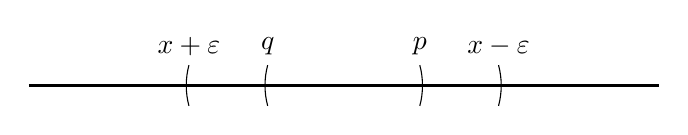
\begin{tikzpicture}
		\draw[thick] (-4, 0) -- (4, 0);
		\draw (2,0) arc [start angle=0, end angle=15, radius=1] node[above] {$x - \varepsilon$};
		\draw (2,0) arc [start angle=0, end angle=-15, radius=1];
		\draw (-2,0) arc [start angle=180, end angle=165, radius=1] node[above] {$x + \varepsilon$};
		\draw (-2,0) arc [start angle=180, end angle=195, radius=1];
		\draw (1,0) arc [start angle=0, end angle=15, radius=1] node[above] {$p$};
		\draw (1,0) arc [start angle=0, end angle=-15, radius=1];
		\draw (-1,0) arc [start angle=180, end angle=165, radius=1] node[above] {$q$};
		\draw (-1,0) arc [start angle=180, end angle=195, radius=1];
	\end{tikzpicture}
	\caption{Question 1.12 Example}
	\label{fig:label}
\end{figure}

\end{document}